\section{Introduction}
A major goal of the Habitable Worlds Observatory, a concept for a mission that
would be the next flagship astrophysics observatory, is to characterize the orbits
and atmospheres of at least 25 potentially habitable worlds \citep{GreatObservatory}. To do this it will use
the direct imaging exoplanet detection technique since it provides the best
opportunity for full spectral characterizations. However, exoplanets are among
the faintest objects that have been the primary targets of an observation and
will require days to weeks of integration time. To complicate matters further,
multiple observations will be required to pin down the orbit of an exoplanet
before deciding on the best time to do a full spectral characterization \citep{horningMinimumNumber2019}.
Allocating the time required for spectral characterizations is therefore
incredibly costly given the considerable cost of construction, operation, and
alternative science objectives for a mission like the Habitable Worlds
Observatory.

Early in the life of a mission, many design decisions are driven by modeling
how the different aspects of a mission impact the science goals of a mission.
For exoplanets this can be seen in papers discussing the tradeoffs between the
diameter of the primary mirror and the number of exoplanets  that will be
detected, often called the "mission yield". Yield modeling studies will be
important to the success of the Habitable Worlds Observatory and two primary
tools have been created to study the mission yield of space-based direct
imaging missions, \code{EXOSIMS}
\citep{savranskyEXOSIMSExoplanetOpenSource2017} and Altruistic Yield
Optimization (AYO) \citep{starkMaximizingExoEarthCandidate2014}. Both tools
were built around calculating the mission yield with no prior information about
the planetary system of the available target stars. However, it is likely that
by the time of launch there will be a considerable amount of information for
some planetary systems.

Considerable effort is being invested into improving the radial velocity (RV)
exoplanet detection method to discover more exoplanets, and it has been
identified as the most promising method to detect Earth-like exoplanets. The
mission concept studies of both HabEx and LUVOIR identified the collection of
precursor RV data as integral to increasing the number of exoplanets detected
\citep{gaudiHabitableExoplanetObservatory2020, TheLUVOIRTeam2019}. An
Earth-like exoplanet's RV signal is on the order of 10 cm/s but current
instruments are typically on the order of 1 m/s RV precision. Because of
this, a number of "Extreme Precision Radial Velocity" (EPRV) instruments capable of detecting Earth-like exoplanets, are being proposed and
studied \citep{Crass2021}.

The most recent study, \citet{morganExplorationExpectedNumber2022a}, showed
that having precise orbital information from RV before launch can improve yield
considerably. \citet{morganExplorationExpectedNumber2022a} showed that EPRV
information reaches the same number of detected exoplanets that a search
without prior information, a blind search, finds in 600 fewer days. This study
is best thought of as an upper bound for the mission yield improvement due to
RV data because it assumed full orbital knowledge. Assuming full orbital
knowledge was done probabalistically based on research on what planets are
likely to be discovered depending on the amount and quality of RV data
collected. This makes it a quick and robust way to determine which planets are
likely to be detected.

The drawback of using full orbital recovery for yield modeling is that fitting
orbits to RV data only estimates certain orbital parameters. A common set of
fitted parameters is period $T$, time of conjunction $T_c$, argument of
periapsis $\omega$, eccentricity $e$, and minimum mass $M_p \sin{i}$. The
minimum mass quantity combines two parameters that impact direct imaging and
estimations of an exoplanet's brightness and location cannot be exact without
separating the planet mass and inclination. Without data from other detection
methods those quantities cannot be separated. An additional complication is
that orbit fits have uncertainties on fitted parameters which should be
accounted for when scheduling observations.

A way of accounting for the inclination and mass ambiguity and uncertainty was
shown in \Cref{cha:first_paper}. The uncertainties from the fitting
process and an inclination prior are used to create a set of orbits that the
planet that created the radial velocity curve is most likely to be on. Then the
probability of detection is calculated, similar to the completeness metric
established in \citet{Brown2005d}, by propagating the orbits in that set and
comparing each orbit's brightness and planet-star separation to a direct
imaging telescope's sensitivity limits.

Fully simulating direct imaging missions with precursor RV requires simulating
the many RV observations that collect RV data for the stars in the direct
imaging target list. Real RV data cannot be used because the full planetary
systems that generate real RV data are unknown. Using the full orbital
knowledge approach also has to face the problem that Earth-like planets can
only be detected with RV if they are around stars with little stochastic
variation in their brightness which is not guaranteed to be the case unless the
target list is restricted to only consider low variability stars
\citep{Crass2021}.

\section{Methods}
To incorporate precursor data realistically we must create synthetic planetary
systems around the stars in the simulation, simulate the collection of RV data,
do blind RV fitting of the RV data to create fits for scheduling, calculate the
probability of detection for each fit during the direct imaging mission, and
finally use the probability of detection information to create a direct imaging
observation schedule, and finally simulate the mission using a direct imaging
mission simulator. The major code pieces are \code{EXOSIMS} for planet
generation and direct imaging observation simulations, \code{RVSearch} for
blind fitting RV data, and the new Python package \code{RVtoImaging} that
handles RV data generation, generating probability of detection data, and
scheduling direct imaging observations. An overview of the software workflow is
shown in \Cref{fig:rv2imgflowchart}.

\begin{figure}
  \begin{center}
    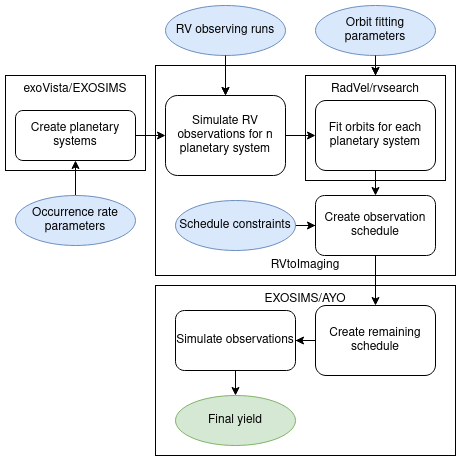
\includegraphics[width=0.95\textwidth]{ch4/figures/flowchartwhite.png}
  \end{center}
  \caption{Framework for simulating the use of precursor radial velocity data
  for direct missions.}
  \label{fig:rv2imgflowchart}
\end{figure}

\code{RVtoImaging} was designed to cache everything that can be used again to
reduce computation time and to include detailed logging information. Inputs are
managed as a set of Python dictionaries from a driver script that is easily
modified to test different RV or direct imaging scenarios.

\subsection{Planetary system generation}

Full "universes" of planetary systems can be generated by \code{EXOSIMS} or
\code{exoVista} \citep{starkExoVistaSuitePlanetary2022}. The universe is then
imported into a Python package, \code{exoverses}, which was created to work as
an intermediary between the different planetary system generators and
\code{RVtoImaging}.

\subsection{RV Dataset}

The RV dataset is composed of user-defined RV surveys (called "observing runs"
in the code) and a set of target stars. These surveys are defined by
\begin{itemize}
  \item Bad weather probability
  \item Exposure time
  \item Minimum and maximum airmass
  \item Minimum number of observations per star
  \item Observatory location
  \item Start and end time
  \item RV precision terms
  \item Observation scheduling scheme
\end{itemize}
\code{RVtoImaging} uses the \code{astroplan} Python package to
determine observability of the target stars for the observatory location and
airmass constraints \citep{morrisAstroplanOpen2018}. 

% The random observation
% scheme takes in an average number of observations per star per year and assigns
% those observations to discrete blocks that are equal in length to the exposure
% time. Observations cannot overlap and stars are only observed once per night.
% The constraint observation scheme is set up to simulate having a set number of
% observing nights. Users define a set number of nights for observation and the
% nights are drawn randomly within the given time frame.

\subsubsection{Scheduling RV observations}

\code{RVtoImaging} currently handles two different RV observation scheduling schemes,
"random" and "constraint". Both require that a target be observable at the time
of observation. The random observing scheme assigns observations on every
available night randomly while respecting observability and only making one
observation per target per night. The constraint observing scheme works based
on maximizing the number of stars above the user defined minimum observations
per star and maximizing the number of observation slots used each night. The
scheduling is done using the Constraint Programming Satisfiability (CP-SAT)
solver from OR-Tools \citep{perronORTools2022}. Each available observation of a
star is assigned a Boolean variable, $b_{i,j,k}$, to represent whether an
observation is made of star $i$ during observation slot $k$ of night $j$. Then
constraints are added to require that each star is observed at most once per
night and each observation time has at most one target star. A Boolean
variable,$B_i$, is defined for each star $i$ such that that $B_i = 0$ if the
star has less than the minimum number of observations assigned and one
otherwise. The objective function given to the CP-SAT solver is
\begin{gather}
  \arg{\max_{b_{i,j,k}}} \left\{ \sum_{i,j,k}\left(
  b_{i,j,k}\right) + \sum_i\left( 100 \cdot B_{i}\right)
  \right\}\\
  \textrm{s.t.}
  \sum_k b_{i,j,k} \; \leq \; 1 \; \forall \; i,j\\
  \sum_i b_{i,j,k} \; \leq \; 1 \; \forall \; j,k
  \label{eq:rv_objective}
\end{gather}
where the 100 is a weighting term to prioritize the distribution of
observations among the target stars. After all observations are assigned by
calling the solver, each night gets a random draw of bad weather, if there is
bad weather then the observations from that night do not occur.

\subsubsection{Simulating RV observations}
After a schedule is created we simulate the observation of the stars. For each
observation we calculate the true anomaly, $\nu$, of all planets in the target
star's system at the time of the observation and calculate the true radial
velocity as 
\begin{equation}
v_s = \sum_i \left(K_i \left(e_i
\cos(\omega_i) + \cos(\nu_i + \omega_i)\right)\right) \,
  \label{eq:system_rv}
\end{equation}
where $K_i$, $e_i$, $\omega_i$ are the RV semi-amplitude, eccentricity, and
argument of periapsis respectively of planet $i$. Each survey is defined
with a number of error terms that are added in quadrature to get a final RV
precision. Then we treat the noise sources as uncorrelated and draw RV errors
for each measurement with the final RV precision as the one $\sigma$ value for
a Gaussian distribution centered on zero. We note that there are
time-correlated noise signals, RV jitter, in real RV data which can be
corrected. However, this is done in a case-by-case basis and is difficult to
scale \citep{guptaTargetPrioritization2021}. Because the primary concern of
this work is to inform direct imaging scheduling, we leave full simulation of
RV errors to future work.

% Additionally, we would be adding time-correlated noise with a Gaussian
% processes and then removing them with the same Gaussian process analysis
% \citep{aigrainGaussianProcess2022}. It is possible to deliberately chose
% different kernel functions for the Gaussian process used in generation and
% the Gaussian process used in fitting to add noise, but it is much more
% straight forward to treat the time-correlated noise terms as a single value
% of RV uncertainty to be defined by the user.

This process of generating RV data is repeated for every scheduled observation in the
survey. Then the full process is repeated for every survey in the
RV dataset. \code{RVtoImaging} is set up so that RV surveys are deterministic
for a given synthetic universe and set of survey parameters, allowing a user to
easily test how different combinations of surveys impact fitting and
ultimately direct imaging scheduling. It is easy to compare how an individual
survey impacts the final fit of a planetary system by adding or removing
it from the script driving the simulation.

\subsection{Blind RV fitting}

\code{RVtoImaging} does a blind search for every star with observations in the
RV dataset. A number of tools exist to do RV fitting, but the need to do systematic blind
searches without any prior information limits the number of applicable tools. The one
best suited for this work is \code{RVSearch} which was created for the
California Legacy Survey \citep{rosenthalCaliforniaLegacy2021}. \code{RVSearch}
is built on top of the \code{RadVel}
library \citep{fultonRadvelRadialVelocity2018}, a Python package that uses
Markov Chain Monte Carlo (MCMC) to fit Keplerian orbits to RV data
with confidence intervals. \code{RVSearch} sets up the log-likelihood function
as \citep{rosenthalCaliforniaLegacy2021} 
\begin{equation}
\ln(\mathcal{L}) = -\frac{1}{2}
\sum_i \left[ \frac{\left(v_i - m(t_i) - \gamma_D\right)^2}{\sigma_i^2} +
\ln\left(2 \pi \sigma_i^2\right)\right]
  \label{eq:likelihoodfun}
\end{equation}
where $i$ is the observation index,
$v$ is the RV measurement, $m$ is the model RV, $\gamma_D$ is the instrument's
offset, and $\sigma$ is the root-mean-square of observation error terms. The
model is defined as 
\begin{equation}
m(t) = \sum_n K(t|K_n,P_n,e_n,\omega_n,T_{c,n}) +
\dot{\gamma}(t-t_0) + \ddot{\gamma}(t-t_0)^2
  \label{eq:rv_model}
\end{equation}
where $n$ is the fitted orbit
index, $K(t|K_n,P_n,e_n,\omega_n,T_{c,n})$ is the RV signal for planet $n$, $P$
is the period, $T_{c,n}$ is the time of conjunction, $\dot{\gamma}$ is a linear
trend term, $t$ is the time of interest, $t_0$ is a reference time, and
$\ddot{\gamma}$ is a quadratic trend term. \code{RVSearch} works by creating a
Bayesian information criteria (BIC) periodogram of the RV data to identifying
the strongest periodic signals. \code{RVSearch} calculates the BIC as 
\begin{equation}
BIC = k
\ln\left(n_{obs})\right) - 2\ln{\mathcal{L}}
  \label{eq:bic}
\end{equation}
where $k$ is the number of free parameters and $n_{obs}$ is the number of
observations. With the strongest periodic signal identified \code{RVSearch}
does a maximum a posterior fit to determine the most likely Keplerian
parameters for the planet that generated the periodic signal. Planets are added
to a collective posterior until there are no periodic signals left that improve
the BIC, or until the \code{RVSearch} posterior reaches a user-defined maximum
number of planets to search for.

After all significant periodic signals in the RV data have been identified,
\code{RVSearch} refines them and determines confidence intervals by performing
an MCMC simulation with all planet parameters free. This MCMC process is done
using the \code{emcee} library \citep{emcee} which is a popular Python
implementation of the affine invariant ensemble sampler \citep{Goodman2010}.
This process is very computationally costly, because the search space increases
considerably with every new planet and the periodogram does a maximum a
posterior fit at every test period with all parameters of previously added
planets free.

\code{RVtoImaging} works on forked versions of \code{RVSearch} and
\code{RadVel} that were created to improve the performance of the original
codes (\url{github.com/CoreySpohn/rvsearch} and
\url{github.com/CoreySpohn/radvel}). The \code{RVSearch} fork was created
primarily because the current \code{RVSearch} package is pegged to
\code{RadVel} version 1.3.8 and does not work with \code{RadVel} versions 1.4.x
which improved performance by vectorizing a number of calculations. Further,
the fork modifies some class attributes so that \code{RVtoImaging} can access
additional sampler information, including whether the MCMC chains converged.
The \code{RadVel} fork has a number of minor optimizations and a major
optimization in the form of a C implementation of the log likelihood function
that uses the fast eccentric anomaly solver from \code{orvara}
\citep{brandtOrvaraEfficient2021}, which is based on
\citet{raposo-pulidoEfficientCode2017}. An experimental feature was added to
RVSearch to allow for the periodogram search to be done without letting all
planet parameters vary which dramatically speeds up the periodogram search.

There are two major bottlenecks in this process. The first is that MCMC does
not scale well with multiple cores because \code{emcee} exits parallelization
every time it checks for convergence. Because of this it is better to spawn
multiple processes that use 5-10 cores each because any benefit gained by
parallelizing the periodogram search is offset by the wasted time in MCMC. The
more limiting bottleneck is that MCMC convergence drops considerably as more
planets are added. An unconverged MCMC run will give biased confidence
intervals which are of primary importance for estimating when a planet is
detectable, so we will not consider unconverged chains valid in this work.
Convergence is rare, less than 20\%, when the number of planets in the search
space is five or more. When running multi-planet fits for yield calculations we
found capping the number of planets in the search to four as a viable option
because it results in a 57\% convergence rate and a standard run time of 30-40
minutes per search when run with 10 cores.

A major drawback of those computational limitations is that, generally, as more
planets are added to the model the parameter distributions of the fitted
planets become better constrained so attempting multi-planet fits without
allowing the search to find as many planets as possible will result in worse
orbital fits. Additionally, by capping the number of planets fitted per system
we limit the number of planets we will consider in the scheduling step,
lowering the maximum yield. This is an unfortunate limitation because it
restricts our ability to fully understand the impact of different RV precision
value. This limitation is a necessary consequence of fitting tools prioritizing
precision over efficiency.

\subsection{Probability of Detection}

Probability of detection is calculated in the manner laid out in
\Cref{cha:accurate_pdet}, which is an adaptation of the "completeness" metric
described in \citet{brownSingleVisitPhotometric2005}. Using the MCMC chains
from the fitting process we generate a representative sample of orbits that are
consistent with the observed RV data for each planet fitted. If the orbits are
an accurate description of the RV signal, we can propagate the orbits in time
and the true planet will be detectable when the orbits are all detectable.
\code{RVtoImaging} is set up to work the "Credible Interval" or the
"Multivariate Gaussian" methods of constructing consistent orbits, since
\Cref{cha:first_paper} showed there is little benefit to only using a single
set of orbital parameters.

Calculating probability of detection relies on a specific set of direct imaging
observatory parameters, since an orbit is considered detectable if it meets the
criteria laid out in \Cref{cha:accurate_pdet}. The
$\Delta\textrm{mag}_0(\alpha, t_{\textrm{int}}, Z, n_\textrm{EZ})$ values are
found for a specific telescope using \code{EXOSIMS}'s
implementation of the minimization routine shown in \Cref{cha:coupling}
. We do not attempt to create
interpolants for all four $\Delta\textrm{mag}_0$ inputs, instead calculating a
2d interpolant that takes in $\alpha$ and $t_\textrm{int}$ values and returns
the $\Delta\textrm{mag}_0$. An interpolant is calculated for a discrete set of
$Z$ values, covering the range of possible $Z$ values for the star during the
telescope's orbit, and a single $n_\textrm{EZ}$ value. Exozodiacal light
brightness is a function of the separation $\alpha$ and drops off with a
$1/r^2$ term as discussed in \citet{starkMaximizingExoEarthCandidate2014}, so
at every separation $\alpha$ we calculate the corresponding exozodiacal light
surface brightness. Then when calculating the $\Delta\textrm{mag}_0$ values at
an observation time $t$ we use the interpolant created with the closest $Z$
value greater than the $Z$ of observing the target star at $t$ and the
user-defined $n_\textrm{EZ}$ value to be assumed in the planetary system. 

% Ideally, we would be assigning the number of $n_\textrm{EZ}$ in the system
% probabilistically for each constructed orbit, but this considerably increases
% the computational load and our knowledge of $n_\textrm{EZ}$ distribution is
% limited. Instead we treat the number of exozodis in the planetary system as
% an input and assume it to be constant when calculating the $P_\textrm{det}$
% values for all planetary systems.

In \code{RVtoImaging} the user defines an \code{EXOSIMS} input script for
telescope parameters, the consistent orbit construction method as defined in
\Cref{cha:first_paper}, a minimum integration time, a maximum integration time,
a start time, and an end time. Then the orbits are repeatedly propagated
between the start and end times and $P_{\textrm{det}}(t, t_{\textrm{int}},
n_\textrm{Z}, n_\textrm{EZ})$ is calculated for integration times spaced
logarithmically between the minimum and maximum. The $P_{\textrm{det}}$
information for all planets around a star are stored as a three dimensional
array that is indexed on the planet number (as assigned during RV fitting),
$t$, and $t_{\textrm{int}}$. The $P_\textrm{det}$ values can then be
interpolated for any set of $t$ and $t_\textrm{int}$ values necessary during
scheduling.

\subsection{Scheduling Observations}
\label{sub:scheduling}

Our aim in this work is to schedule observations of the fitted planets in a way
that is consistent with the observation strategies outlined in the HabEx and
LUVOIR studies \cite{gaudiHabitableExoplanetObservatory2020,TheLUVOIRTeam2019}.
They outlined a multi-tiered process that begins by using the telescope's
detection observing mode, as opposed to the observing mode for atmospheric
characterization, to better resolve the orbits of planets in the initial
portion of the mission. Prior work has shown that it takes 3-4 direct imaging
observations to determine an exoplanet's orbit to 10\%
\citep{bluntOrbitsImpatient2017}, and fewer are required when precursor data
exists \citep{gaudiHabitableExoplanetObservatory2020}. Further, it's important
to try and space out observations of a planet, as gathering 3 observations of
an Earth-like planet on 3 consecutive days will result in a considerably worse
fit than 3 observations made months apart. We use this information to drive our
scheduling task, attempting to get decent orbital coverage of as many fitted
planets as possible to simulate the initial orbit fitting part of the mission.

\subsubsection{The CP-SAT Solver}

Scheduling is done with a constraint programming tool, the CP-SAT solver from
OR-Tools \citep{perronORTools2022}. CP-SAT is built to transform a constraint
programming (CP) problem into a satisfiability (SAT) problem
\citep{knuthSatisfiablility2018}, using the Lazy Clause Generation method
outlined in \citet{feydyLazyClause2009a}, and then solve the model using a SAT
solver.

% Most of the information contained in this section has
% been gathered by searching through the OR-Tools documentation
% \url{developers.google.com/optimization}, the project GitHub, and various video
% presentations given by the developers.

Constraint programming is defined by a set of variables and a set of
constraints. Each variable is assigned a finite range of values and constraints
are made on some subset of all the defined variables
\citep{shawConstraintProgramming2002}. The most common constraints are equality
relations between variables, however modern solvers provide many useful
abstractions such as conditional constraints, absolute value constraints, and
multiplication of variable constraints. Constraint programming is built around
the idea of finding a feasible solution rather than a necessarily optimal
solution because it is meant to work with very large sets of possible solutions
where finding an optimal solution is not computationally feasible. This does
not mean that it is unable to handle optimization though, as an objective
function to be minimized or maximized can be defined based on the variables in
the problem.

% Satisfiability problems consist of finding a variable assignement  fundamental 

% Using the CP-SAT solver is a combination of constraint programming, metaheuristics,



\subsubsection{Decision variables}

Our decision variables are Booleans $x_{i, t, t_{\textrm{int}}}$ that are true
(one) when star $i$ is observed starting at time $t$ with integration time
$t_{\textrm{int}}$, and false (zero) otherwise. Large scheduling problems
cannot be practically solved with continuous variables, so \code{RVtoImaging}
discretizes the times $t$ between the mission's start and end into discrete
observing blocks determined by the user input minimum block size, mission start
time, and mission end time. Then the integration times $t_{\textrm{int}}$ are
set as user-defined multiples of the minimum observing block size.

To improve performance we take a number of steps to avoid creating $x_{i, t,
t_{\textrm{int}}}$'s that serve minimal purpose. Using the \code{EXOSIMS}
script that created the $P_{\textrm{det}}$ values we determine the keep-out
times, the times when the target star is in a region of the sky where light
from a solar system body makes exoplanet observations impossible, and only
create an $x_{i, t, t_{\textrm{int}}}$ when the star is not in keep-out. The
user sets a $P_{\textrm{det}}$ threshold and we create no $x_{i, t,
t_{\textrm{int}}}$ when all of the fitted planet's $P_{\textrm{det}}$ are below
the threshold. We loop through $t_{\textrm{int}}$ values from shortest to
longest and only create a new $x_{i, t, t_{\textrm{int}}}$ Boolean when the
increase in integration time would result in more of the star's planets being
above the $P_{\textrm{det}}$ threshold. The CP-SAT
solver only works on integer values, so we multiply all $P_{\textrm{det}}$
values by a constant, user-defined coefficient and cast the values as integers.
While a large coefficient will more accurately represent the true
$P_{\textrm{det}}$ values, the use of a threshold does not require it, and we
have found a coefficient of 100 to be sufficient. An alternative objective
function built to maximize $P_{\textrm{det}}$ would depend on the coefficient
used.

\subsubsection{Constraints}

The main benefit of the CP-SAT solver is its flexibility regarding constraints.
Two obvious constraints for this work are that observations must be scheduled
between the start and end of the mission and that observations must be
separated by at least the observation overhead time. Another constraint is the
maximum number of observations of a single star. Flexibility in how long we
wait between observations of a star is important for orbital coverage, so
\code{RVtoImaging} takes as input a minimum and maximum wait time between observations
of a star. We want to tailor the wait time to the fitted systems, so we start
with a wait time of one quarter of the period of the planet with the shortest
fitted period. That wait time is used if it is within the range of the min and
max wait times, and is constrained to the bounds if they are exceeded.

Adding all of these constraints as linear equations over the Booleans $x_{i, t,
t_{\textrm{int}}}$ gets complicated quickly. To make constraints easier to
express we use an abstraction that OR-Tools provides called an "Optional
Interval Variable", which are defined by an integer "start" variable
$c_\textrm{start}$, an integer "size" variable $c_\textrm{size}$, and a Boolean
"active" variable $c_\textrm{active}$. These intervals can be made to represent
an observations by mapping the discrete $t$ values to the $c_\textrm{start}$
variable and the discrete $t_\textrm{int}$ values to the $c_\textrm{size}$
variable. Interval variables map onto observations of a single star. Intervals
are effectively "off", not considered in constraints, when their
$c_\textrm{active}$ variable is false. We only create as many intervals as is
required per star, the minimum value between the user-set maximum observations
per star and the product of the number of fitted planets around a star and the
requested number of observations per planet. We connect the decision variables
to the interval variables using "channeling constraints", intermediate Boolean
variables that allow if-then style relationships. This forces a decision
variable, $x_{i, t, t_{\textrm{int}}}$, to be true when an interval's
$c_\textrm{active}$ variable is true and its $c_\textrm{start}$ and
$c_\textrm{size}$ values match the decision variable's $t$ and $t_\textrm{int}$
values.

\subsubsection{Objective Function}

The decision variables $x_{i, t, t_{\textrm{int}}}$ are used because they can
be correlated to the $P_\textrm{det}$ values much more easily than the interval
variables in the final objective function. Our goal here is not to simply
maximize the $P_\textrm{det}$ values, it is to improve the fits of as many
planet orbits as we can. Because of this we set up an integer variable for each
fitted planet, $b_\textrm{planet}$, that is equal to the number of observations
of the planet's star that occur at a time when the fitted planet is at or above
the user-set $P_\textrm{det}$ threshold. The $b_\textrm{planet}$ variables are
bounded at the user-input number of observations per planet and are calculated
using a channeling constraint
\begin{equation}
  b_j = \sum_{t, t_\textrm{int}}(x_{i, t, t_\textrm{int}}P_{\textrm{det}, j, t, t_\textrm{int}} >= P_\textrm{thresh})\\
  \label{eq:bplanet}
\end{equation}
and is constrained to be between 0 and 3. The final objective function is stated as 
\begin{gather}
  \arg\max_{x_{i,t,t_\textrm{int}}}{\left\{ \Sigma\left(W \cdot
  b_\textrm{j}\right) - \Sigma\left( c_\textrm{active}\right) - \Sigma\left(
  c_\textrm{size}\right) \right\}}\\
  \textrm{s.t.} \; \sum_{t,t_\textrm{int}} x_{i,t,t_\textrm{int}} \; \leq \; n_i \; \forall \; i\\
  \sum_{i, t_*\in[t,t+t_\textrm{OH}], t_\textrm{int}} x_{i,t_*,t_\textrm{int}} \; \leq \; 1 \; \forall \; t\\
  \sum_{t_*\in[t,t+t_{i,\textrm{wait}}], t_\textrm{int}} x_{i,t_*,t_\textrm{int}} \; \leq \; 1 \; \forall \; i, t
 \label{eq:final_obj_function}
\end{gather}
where $W$ is a weight term such that the $b$ terms dominate, $n_i$ is the
number of planets fitted around star $i$ multiplied by the number of request
observations per planet and constrained to the maximum number of observations
per star, $t_\textrm{OH}$ is the required overhead time to switch targets, and
$t_{i,\textrm{wait}}$ is the required time to wait before revisiting star $i$.
The $c_\textrm{active}$ terms are included in the objective function to prevent
observations with no benefit from being included. The $c_\textrm{size}$ terms
are included in the objective function to reduce the integration times if doing
so does not affect the $b_\textrm{planet}$ term. With the constraints and the
objective function added to the CP-SAT model we can use the CP-SAT solver to
find an observation schedule that maximizes the objective function.

\subsubsection{Simulating Observations}

With a schedule created we can simulate observations of the synthetic planetary
systems that created the synthetic RV data by importing the systems into an
\code{EXOSIMS} \code{SimulatedUniverse} module and then running an
\code{EXOSIMS} mission simulation. The same \code{EXOSIMS} input script that
was used to generate the $P_\textrm{det}$ values is used for the mission
simulation. This may come across as overfitting, given that we are using the
same tool when estimating the probability of detection and determining true
detectability. This is unavoidable for our purpose as mission simulation
software is continually evolving to include as much detail as possible to
simulate a direct imaging mission and represents our current models of direct
imaging. It will be a continually moving target to keep the probability of
detection model up to date with our current understanding of what factors drive
a planet's detectability. As they become more complex so must the probability
of detection model.

\section{Results}

We populated every star in the NETS target list
\citep{guptaTargetPrioritization2021}, a set of 100 high priority radial
velocity targets, with a planetary system drawn from the
\citet{dulzJointRadialVelocity2020} occurrence rates, redrawing the system if
an Earth-like planet was not included as a best-case scenario to test how well
the scheduler performs with a large number of possible targets. The planets
outside of the habitable zone were not included in the radial velocity
calculations as fitting multi-planet systems increases the computation time by
many orders of magnitude and in a real-life scenario there would be manual
vetting of the individual fits instead of strictly blind searches. The radial
velocity data was generated using a hypothetical EPRV instrument with
$\sigma_\textrm{RV} = 3$ cm/s at the Keck observatory. We gave the radial
velocity instrument 100 observing nights per year for 5 years, an exposure time
per target of 20 minutes which is roughly in line with the average NEID
exposure time and overhead time of 18.74 minutes
\citep{guptaTargetPrioritization2021}. We set the bad weather probability to
zero for the work to simulate a mission which would be allowed to reschedule
observations if weather prohibited observing on a night. We assume that the RV
observations continue right up until the mission launch to eliminate dispersion
error which was described in \Cref{cha:first_paper}. We set a schedule
optimization goal of 100 observations per target star for the radial velocity
scheduler and allowed the scheduler 10 minutes to run.

After simulating the observations and generating the radial velocity fits as
described above we calculated the probability of detection values using 10000
orbits constructed with the "credible interval" orbit construction method
described in \Cref{cha:first_paper}. The orbits were propagated for two years,
the approximate time allocated for the Earth-like survey by the HabEx team
\citep{gaudiHabitableExoplanetObservatory2020}. The probability of detection
values were calculated for 19 integration times spaced logarithmically between
the minimum integration time of one hour and the maximum integration time of 30
days. The observatory was assumed to be on an L2 orbit and the local zodiacal light
was calculated as a function of the observation time and the star's position using
the method from \Cref{sub:zodi}.
The assumed $n_\textrm{EZ}$, for $P_\textrm{det}$ calculations, in the
planetary systems was treated as a constant value in these simulations but the
change in surface brightness as a function of separation was accounted for in
our estimation of $P_\textrm{det}$.

Finally the direct imaging scheduler was allowed integration times of 6 hours,
1 day, 5 days, 10 days, and 30 days. The planet was to be considered detectable
if the probability of detection was equal to or above 0.95 and each planet was
to be observed 3 times when possible. Then we set the minimum required wait
time to re-observe a star to 10 days and the maximum required wait time to a
quarter of a year. The scheduler was allowed to run for two hours.

\begin{figure}
  \begin{center}
    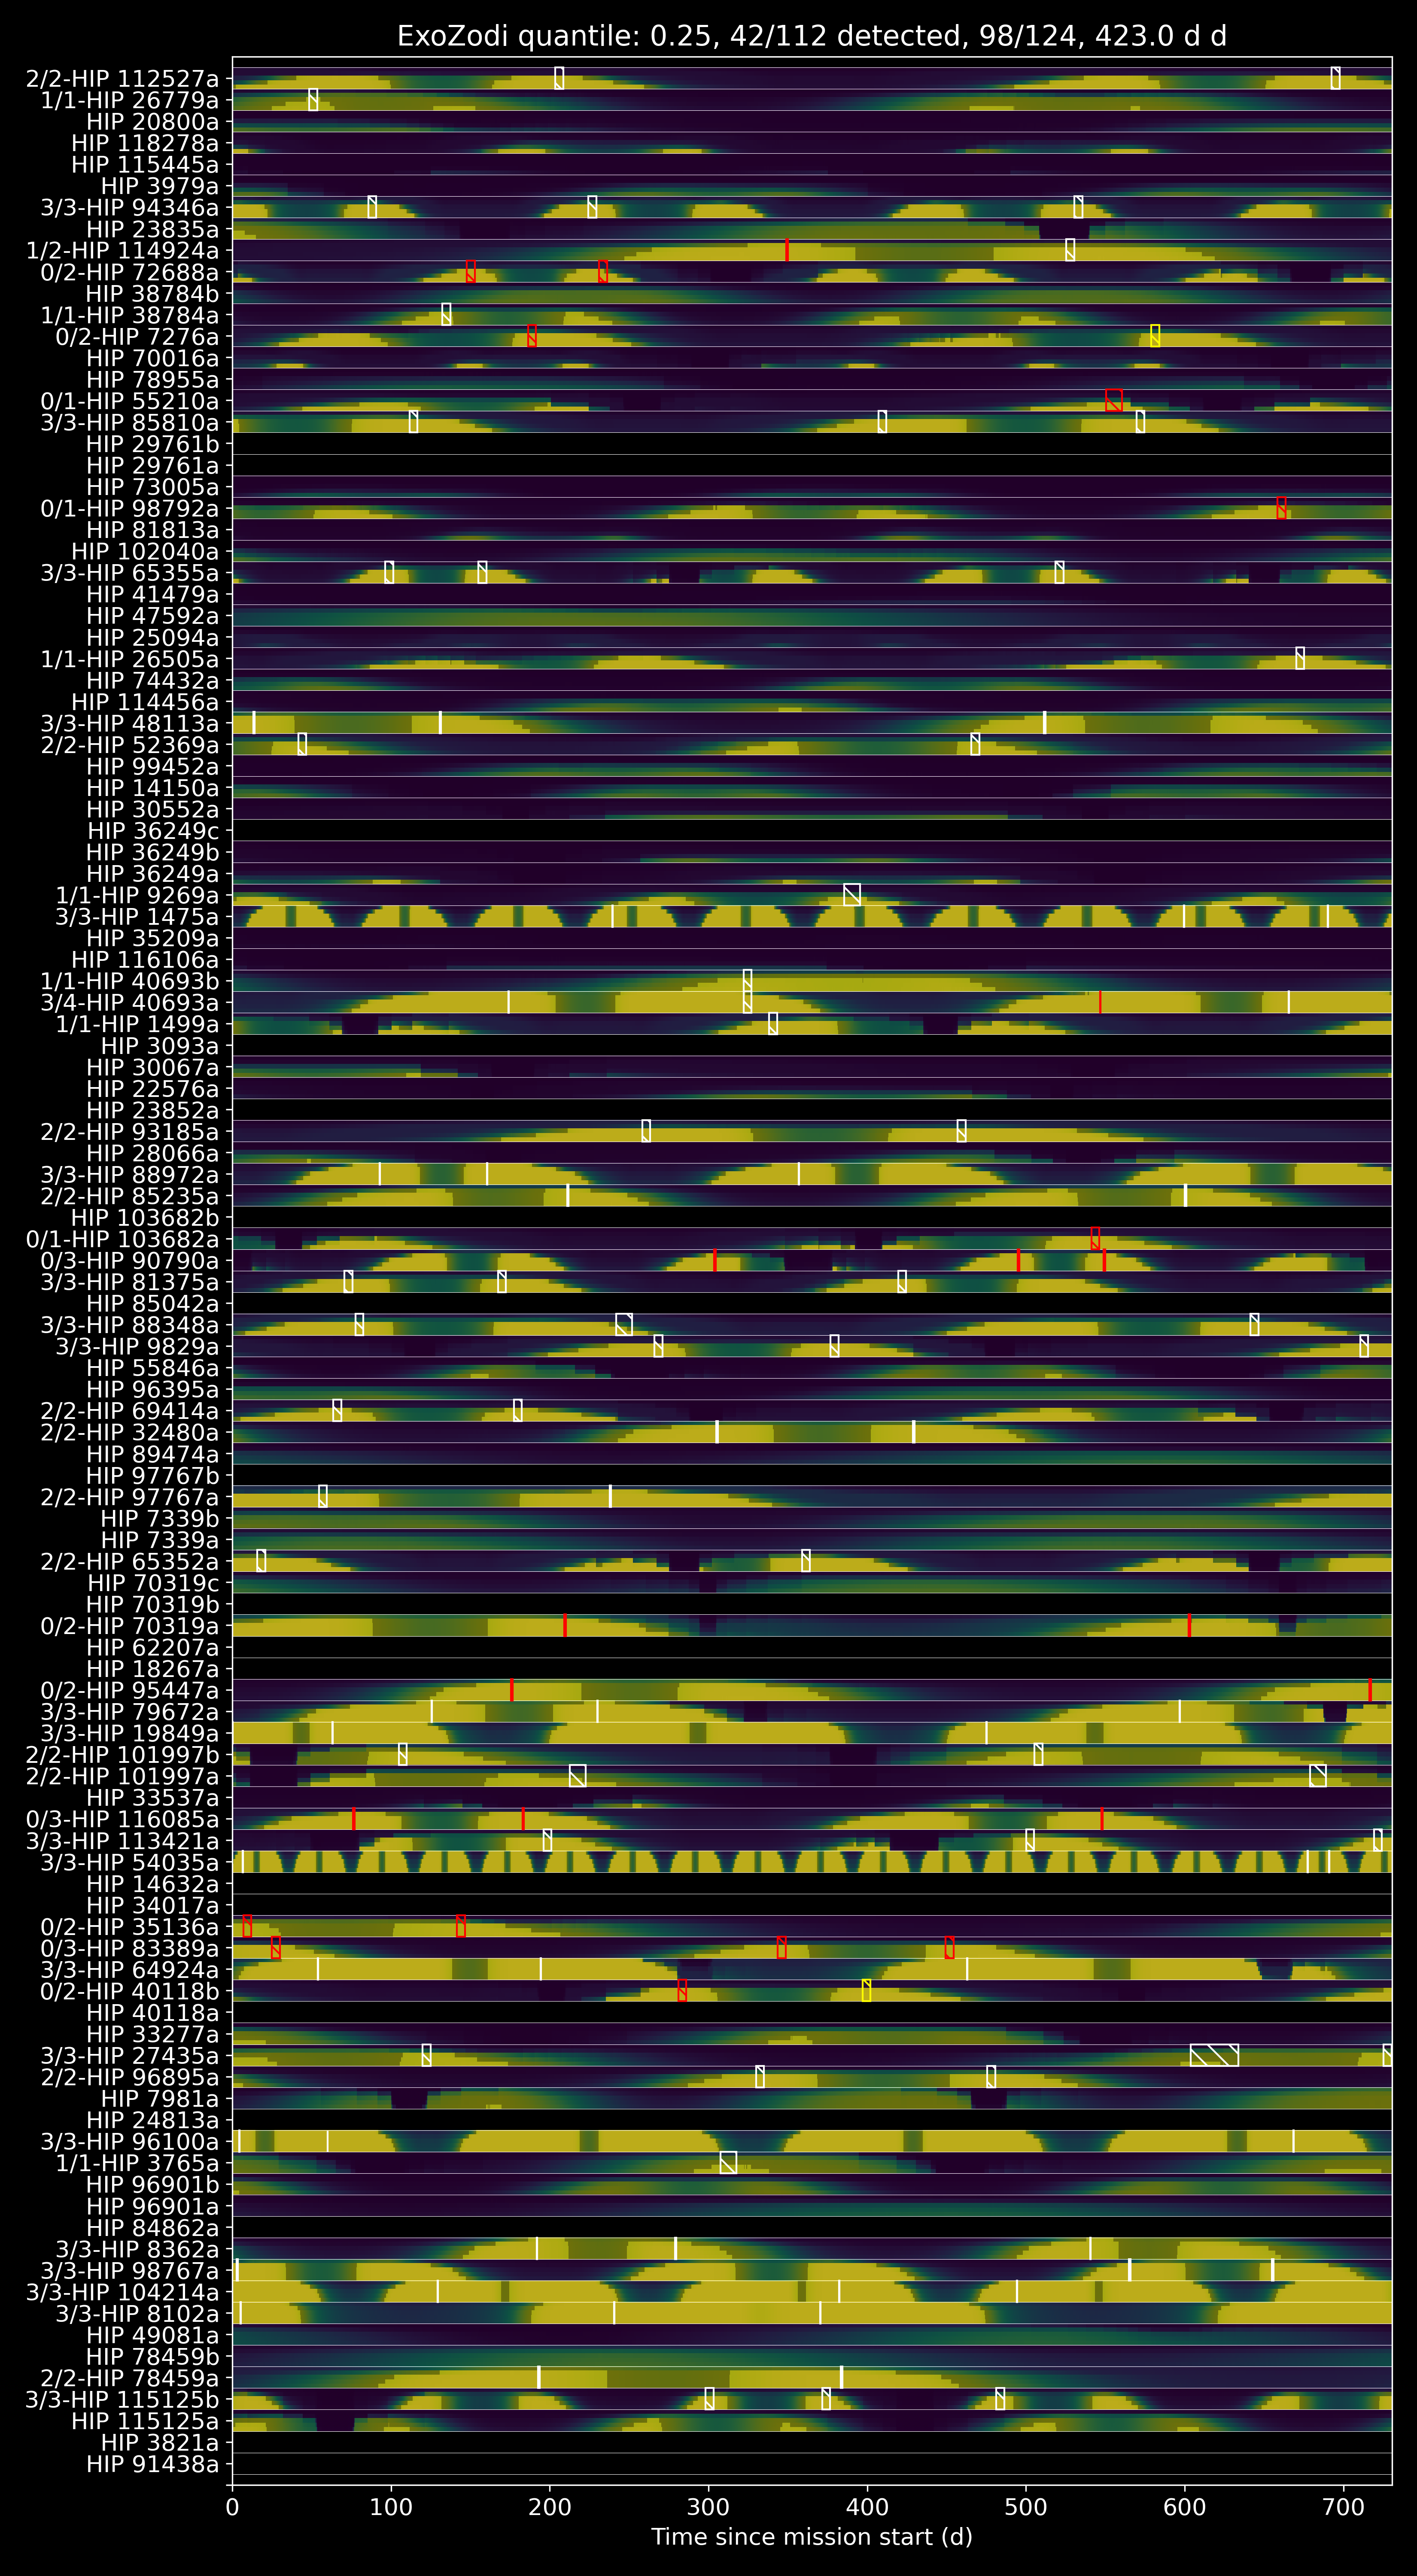
\includegraphics[height=0.9\textheight]{ch4/figures/example_schedule.png}
  \end{center}
  \caption{
    Schedule created based fits of 3 cm/s EPRV data on 97 stars populated with
    Earth-like planets. (Remaking this plot today, harder to change than the others).
  }
  \label{fig:schedule}
\end{figure}

\begin{figure}
  \begin{center}
    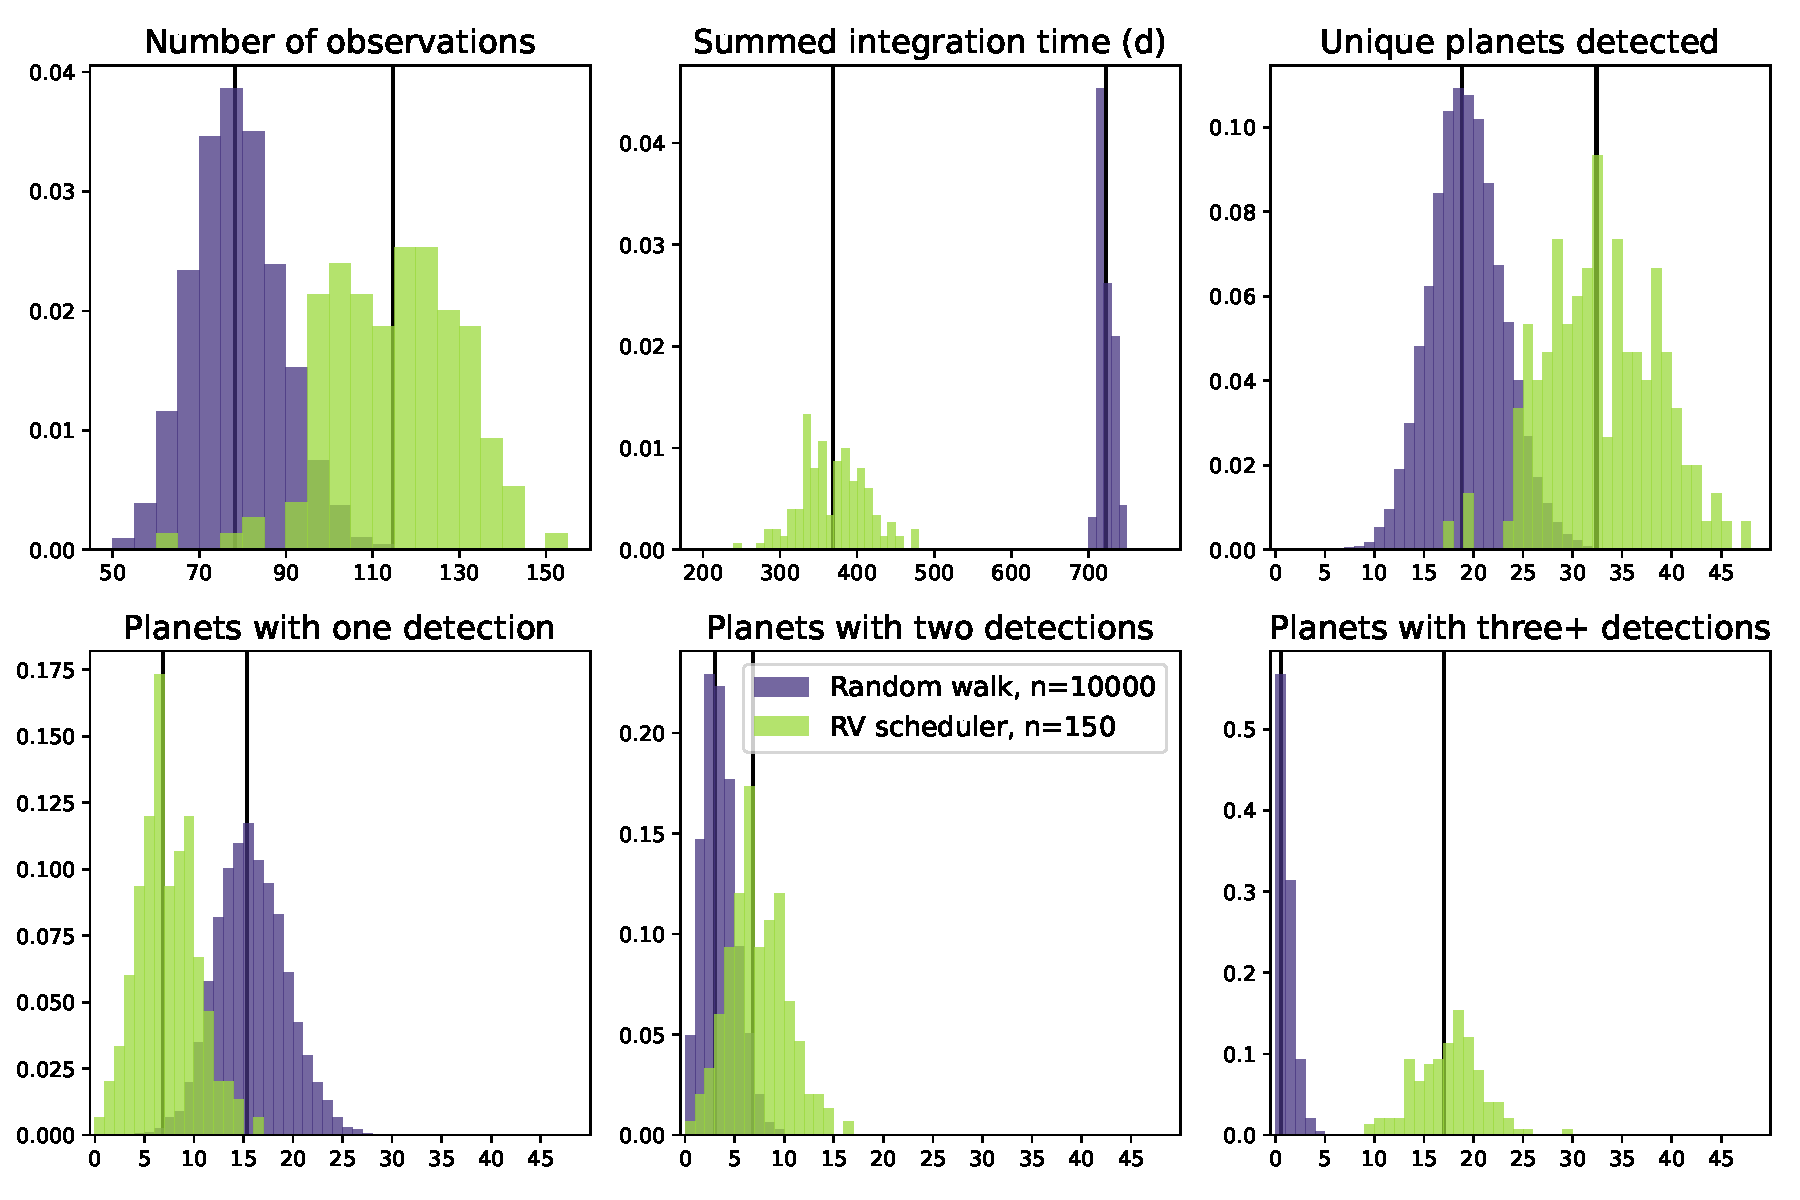
\includegraphics[width=1\textwidth]{ch4/figures/final_results.pdf}
  \end{center}
  \caption{Comparison between the RV scheduler and a random walk schedule.
  All stars in the NETS target list were populated with an Earth-like planet,
  observed with a 3 cm/s RV instrument, and then had observations scheduled
  using the RV scheduler described in \Cref{sub:scheduling}. Top row shows
  summary results of the number of observations, the total integration time
used, and the number of unique planets found when simulating the created
schedule. The bottom row splits the top right plot out to differentiate how
many unique planets had only one detection, how many had two detections, and
how many had three or more detections. The vertical lines represent the mean values
for the distributions. This plot shows that the RV scheduler is able to detect
more planets in an efficient manner. The RV scheduler succeeds in getting $\sim$17
unique planets detected three or more times during the course of the two year
mission which is a strong result for orbit fitting purposes.}
  \label{fig:randomwalkhist}
\end{figure}

An example schedule is shown in \Cref{fig:schedule}, where 42 of the 112
planets was detected at least once, 124 observations were scheduled, and 98 of
the scheduled observations were successful. In total the scheduler used 423
days of integration time out of the allowed two years. It is difficult to find
an analogous comparison in literature to the case we are showing, as previous
studies of RV knowledge fixed the positions of the planets to be the same for
all observations, used a much larger target list, and focused on full
characterization which is not included in this
work \citep{morganExplorationExpectedNumber2022a}. Because of this we compare
our schedule to a random walk scheduler, where we use the same set of planets
and telescope parameters and simulate a mission using a random walk scheduler. When determining
which star to observe the random walk scheduler picks randomly from the stars
that are observable at the current mission time. After a star is picked the
scheduler randomly selects an integration time from the same set of discrete
integration times used by the CP-SAT scheduler and simulates the observation.
This process is repeated until an observation would end after the mission's
end time.
% randomly for the full mission time. The integration times per target star were
% chosen such that instrument could reach $\Delta\textrm{mag}=25$. 

We show 100 full simulations compared to 10000 random walks in 
\Cref{fig:randomwalkhist}. Our scheduler used about half as much integration
time as the random walk and was able to detect approximately 10 more planets
per simulation. It also dramatically out performs the random walk scheduler
in reaching three observations in the allowed mission time.

To test the impact of the precision $\sigma$ and the assumed number of zodis in
a planetary system on the scheduler we ran the same situation without redrawing
until an Earth-like planet is in a system. In this way we end up with fewer
total fits, based on the occurrence rate of Earth-like planets,
$\eta_{\oplus}$, which we set to 0.24 in line with
\citet{dulzJointRadialVelocity2020} occurrence rates which was also used in the
EPRV study \citep{morganExplorationExpectedNumber2022a}. We tested the
scheduler for 5 $\sigma$ values (0.1, 0.07, 0.05, 0.03, 0.01 m/s) and 5
$q_\textrm{EZ}$ values (0.05, 0.25, 0.5, 0.75, 0.95) where the $q_\textrm{EZ}$
values map to an $n_\textrm{EZ}$ quantile from the the occurrence rates derived
in \citet{ertelHOSTSSurvey2020}.

The results are shown in \Cref{fig:sigma_nEZ_impact_plots} where the impact of
the $\sigma$ value on the number of exo-Earths fitted is clearly demonstrated.
We see that if a 3 cm/s precision is reached, the value used in the EPRV study
\citet{morganExplorationExpectedNumber2022a}, then we can fit the orbits of
approximately 80 percent of the Earth-like planets. However, if we are limited
to 10 cm/s we will only expect to fit 40 percent of the Earth-like planets. By
then simulating the probability of detection, scheduling, and observation
process calculations we can study how the different $\sigma$ values impact
observation success rate and we see little effect. The $\sigma$ values strongly
correlate to the percentage of planets detected, which is unsurprising given
that fewer orbits are fitted.

The assumed $n_\textrm{EZ}$ has a positive relationship with the observation
success rate and a negative relationship on the mission yield past the 50th
$n_\textrm{EZ}$ quantile. This shows an interesting trade space where we can
better guarantee the success of an individual observation if we assume high
levels of exozodi, but this approach ultimately has a negative impact on the
total yield of the mission.

% \begin{figure}
%   \begin{center}
%     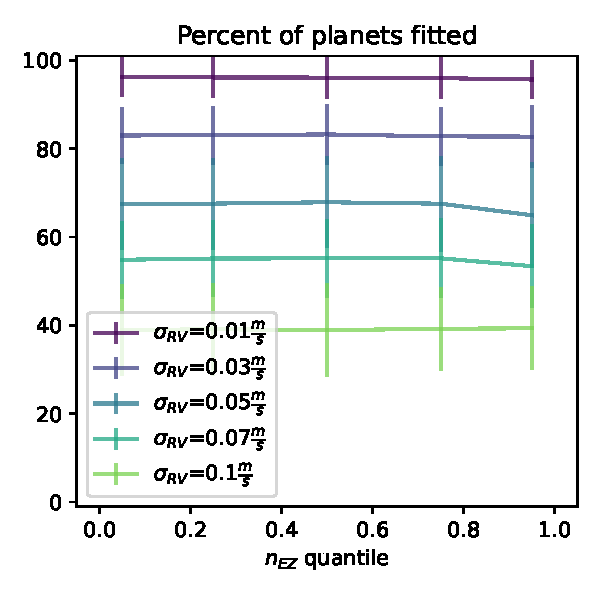
\includegraphics[width=0.9\textwidth]{ch4/figures/percent_fitted.pdf}
%   \end{center}
%   \caption{
%     Impact of $\sigma$ on the number of planets in the simulated universe that
%     are fitted based on the simulated RV data. This can be used to estimate the
%     number of planets that the scheduler will have to account for when given
%     a simulated universe.
%   }
%   \label{fig:sigma_percent_fitted}
% \end{figure}
\begin{figure}
  \begin{center}
    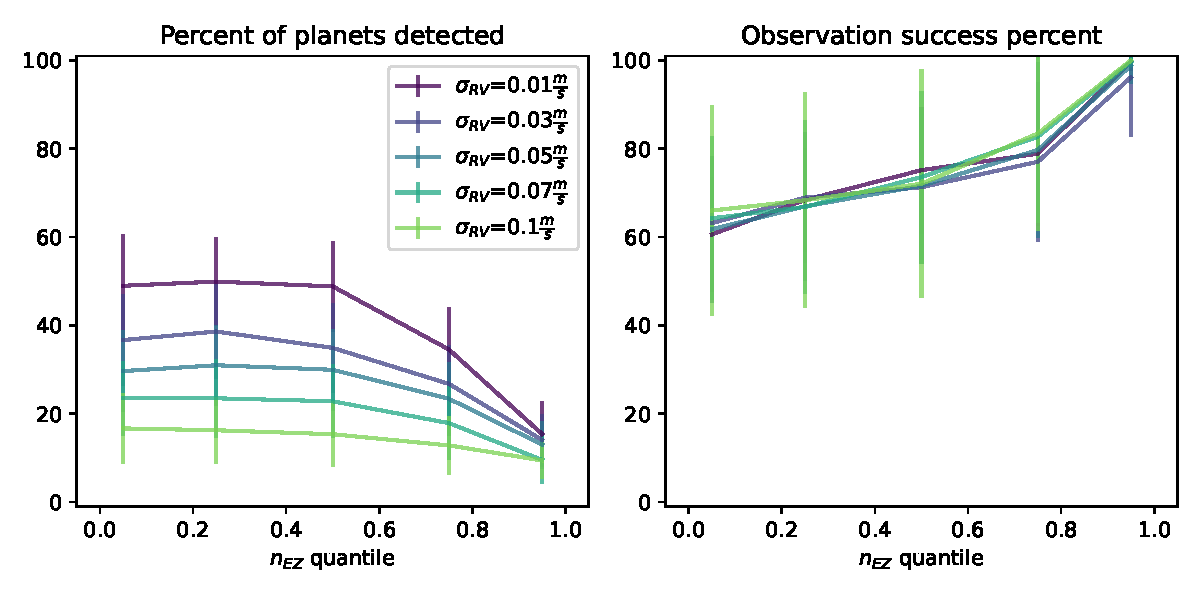
\includegraphics[width=0.9\textwidth]{ch4/figures/succes_rate_vs_percent_detected.pdf}
  \end{center}
  \caption{
    Impact of assumption on $\sigma$ and exozodi on scheduler results. The left plot shows
    that for high assumed values of $n_\textrm{EZ}$ the number of planets detected decreases.
    The right plot shows that when high values of $n_\textrm{EZ}$ are used observations are
    more likely to succeed. Together this plot shows that a direct imaging mission schedule
    will have to decide on whether it is worth assuming large amounts of exozodiacal dust
    to guarantee observations are successful or if it is more important to detect as many
    planets as possible while potentially missing planets in dusty planetary systems.
  }
  \label{fig:sigma_nEZ_impact_plots}
\end{figure}

\section{Conclusion}

In this chapter we have demonstrated a method of using constraint programming
to calculate an observing schedule that allows for dynamic variations in the
integration time and observation time for every planet with precursor radial
velocity data. To validate the scheduler we created a tool called
\code{RVtoImaging} that realistically simulates the RV data collection and
fitting process, calculates the probability of detection for a given orbit fit
and direct imaging telescope, schedules observations based on that data, and
then uses mission simulation software to test the scheduled observations. We
showed that our scheduler dramatically out performs a random walk scheduler.
This work proves that we can use the probability of detection metric to
schedule direct imaging observations of exoplanets detected via radial velocity
and it shows how precursor data can be incorporated in direct imaging mission
yield modeling. Further, efficient scheduling in the manner described will
improve the science yield of a direct imaging mission in meaningful ways.

By creating a flexible framework that does full simulations of the RV
observations and fitting process we have created a tool that can answer many
interesting questions in the use of precursor science for a flagship direct
imaging mission such as the Habitable Worlds Observatory. We used a relatively
simple setup in this chapter: a single survey, no bad weather, only
planets in the habitable zone, and RV observations were continued until the
direct imaging mission launch. Future work will be on more complicated
scenarios, such as: how many EPRV observations of a planetary system are
required to accurately calculate probability of detection, how does the
planetary occurrence rate model impact which planets are ultimately fitted via
radial velocity, how do different RV orbit fitting tools compare, what
synergies exist when scheduling both RV and direct imaging observations for a
combined target list.

